\documentclass[../main/main.tex]{subfiles}

\begin{document}

\newpage
\chapter{Testing}

\section{Iterative Testing}
I have been playtesting the program throughout the development process to find any bugs and fix them accordingly. However, a few issues have required additional measures.

\subsection{Minimax}
Since minimax is recursive algorithm, debugging it has proven a challenge. I have therefore configured the Python \lstinline{logging} library to help collect information on the minimax tree for every function call.

\noindent\verb|base.py|
\lstinputlisting[firstline=27, lastline=51, caption=BaseCPU Method for logging minimax statistics]{../../data/states/game/cpu/base.py}

\subsection{Migrations}
To correct errors made to the \lstinline{games} table, since recreating it would mean deleting all existing games, I have opted to use migrations to fix bugs by editing the table schema, as shown in Section \ref{sec:migrations}.

\section{Unit Tests}
\subsection{Board Evaluator}
To test every aspect of the evaluation function, I have set up some unit tests with custom positions using my editor screen. These positions are designed to test every aspect of the evaluation, along with some obviously imbalanced positions to test the overall accuracy of the evaluation function. All positions are set up to give an advantage to the blue player.

\begin{longtable}[c]{l|l|l|l}
    \toprule
    \textbf{Evaluating} & \textbf{FEN string} & \textbf{Score} & \textbf{Passed}\\
    \midrule
    \endhead

    Material & \verb|sc9/10/10/4paPa4/5Pa4/10/10/9Sa b| & 124 & \checkmark\\
    Position & \verb|sc9/4nanana3/10/10/10/4NaNaNa3/10/9Sa b| & 66 & \checkmark\\
    Mobility & See footnote\footnote{scpapa7/papapa7/papapa1Pa1Pa1Pa1/10/4Pa1Pa1Pa1/10/4Pa1Pa3/9Sa b} & 196 & \checkmark\\
    King Safety & \verb|sc4fa3pa/10/10/10/10/10/10/5FaPa2Sa b| & 3 & \checkmark\\
    Combined & See footnote\footnote{scnc1fcncpbpb3/pa9/pb1pc1rbpa3Pd/1Pc2Pd4Pc/2Pd1RaRb4/10/7Pa2/2PdNaFaNa3Sa b} & 437 & \checkmark\\

    \bottomrule
    
\caption{Board evaluator test results}
\label{tab:testing-evaluator}
\end{longtable}


\subsection{CPU}
Similarly, to evaluate the strength of my CPU, I have setup some custom positions that I already know the best continuation of, and run each CPU engine on them to test if they can solve it.

\begin{longtable}[c]{l|l|l|l}
    \toprule
    \textbf{Description} & \textbf{FEN string} & \textbf{Best Move} & \textbf{Passed}\\
    \midrule
    \endhead

    Mate in 1 & \verb|sc9/pafa8/Fa9/10/10/10/10/9Sa b| & Rotate J3 clockwise & \checkmark\\
    Mate in 1 & \verb|sc9/10/10/10/8faRb/8FaRb/10/9Sa b| & Move J3 to J2 & \checkmark\\
    Mate in 3 & \verb|sc9/10/10/8Ra1/7FaRafa/8RaRa/9Ra/9Sa b| & Move J2 to I1...\footnote{2. \lstinline{Move J4 to J5} 3. \lstinline{Move J3 to I2}} & \checkmark\\
    Mate in 3 & \verb|sc5fcnc2/4Pa4Pc/3pb6/2Pc2ra1pb2/10/pb9/7Pa2/2PdNaFa4Sa b| & Move E7 to F7...\footnote{2. \lstinline{Rotate anticlockwise H8} 3. \lstinline{Move F7 to G7}} & \checkmark\\
    Escape Mate & \verb|sc9/10/10/10/8faRb/8FaRb/10/9Sa b| & Move J3 to J2 & \checkmark\\
    Win Material & \verb|sc9/10/10/10/8faRb/8FaRb/10/9Sa b| & Move J3 to J2 & \checkmark\\

    \bottomrule
    
\caption{Transposition Table CPU test results}
\label{tab:testing-cpu}
\end{longtable}

I have also personally played against the CPU engines to gauge its strength in a realistic setting. The results are shown below:

\begin{longtable}[c]{c|c}
    \toprule
    \textbf{Me} & \textbf{CPU}\\
    \midrule
    \endhead

    2 & 5\\

    \bottomrule
    
\caption{Score of me vs CPU (I am very bad)}
\label{tab:me-cpu}
\end{longtable}

\begin{longtable}[c]{c|c}
    \toprule
    \textbf{Mr Myslov} & \textbf{CPU}\\
    \midrule
    \endhead

    1 & 6\\

    \bottomrule
    
\caption{Score of Mr Myslov vs CPU (Mr Myslov is even worse)}
\label{tab:myslov-cpu}
\end{longtable}

\subsection{Shadow Mapping}
To test the shadow mapping algorithm, I have set up some occluding objects togehter with a light source. Since visuals are subjective, me and my client have deemed the following results to be adequate.

\begin{figure}[H]
    \centering

    \begin{subfigure}[b]{0.3\columnwidth}
    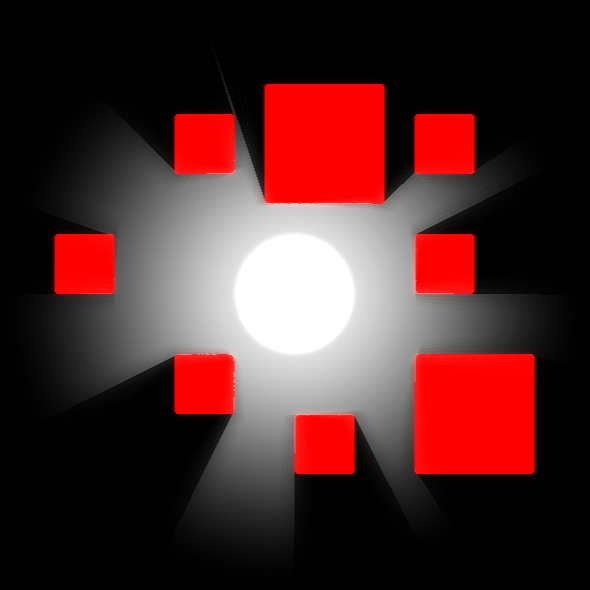
\includegraphics[width=\columnwidth]{../testing/assets/rays_example_1.png}
    \end{subfigure}
    \begin{subfigure}[b]{0.3\columnwidth}
    
\includegraphics[width=\columnwidth]{../testing/assets/rays_example_2.png}
    \end{subfigure}
    \begin{subfigure}[b]{0.3\columnwidth}
    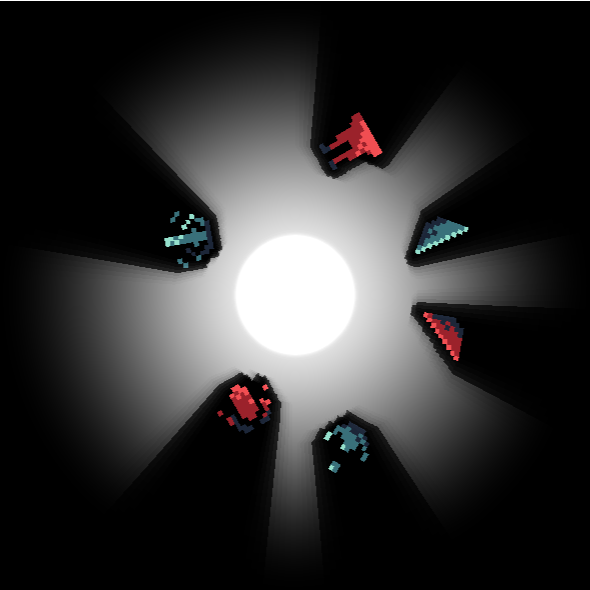
\includegraphics[width=\columnwidth]{../testing/assets/rays_example_3.png}
    \end{subfigure}

    \caption{Shadow mapping algorithm test (softShadow=0.5, radius=0.5)}
    \label{fig:rays-examples}
\end{figure}

\section{Final Tests}
\subsection{Objective 1}
All laser chess game logic should be properly implemented.

\begin{longtable}[c]{l|p{0.35\columnwidth}|p{0.35\columnwidth}|l}
    \toprule
    \textbf{No.} & \textbf{Input} & \textbf{Output} & \textbf{Passed}\\
    \midrule
    \endhead

    1 & Laser fires on piece & Piece reflects laser & \checkmark\\
    2 & Select piece and press rotate clockwise button & Piece rotates clockwise & \checkmark\\
    3 & Select piece and adjacent empty square & Piece moves to adjacent square & \checkmark\\
    4 & Blue player makes a move & Next move is made by red player & \checkmark\\
    5 & Make move & Laser reflects off pieces correctly & \checkmark\\
    6 & Position piece with non-reflecting side facing laser & Piece is destroyed & \checkmark\\
    7 & Move Pharoah in front of player & Game displays game over screen & \checkmark\\
    8 & Repeat same position three times & Game displays game over screen & \checkmark\\

    \bottomrule

\end{longtable}

\subsection{Objective 2}
Save or load game options should be implemented.

\begin{longtable}[c]{l|p{0.35\columnwidth}|p{0.35\columnwidth}|l}
    \toprule
    \textbf{No.} & \textbf{Input} & \textbf{Output} & \textbf{Passed}\\
    \midrule
    \endhead

    9 & Click on copy FEN string button in editor or browser screen & Position formatted as FEN string copied to clipboard & \checkmark\\
    10 & Enter browser screen & Program shows list of past games to be scrolled through & \checkmark\\
    11 & Click on previous or next move button in review screen & Board undoes or applies move & \checkmark\\
    12 & Enter review screen & Program displays list of past moves, winner and move number& \checkmark\\

    \bottomrule

\end{longtable}

\subsection{Objective 3}
Other board game requirements should be implemented.

\begin{longtable}[c]{l|p{0.35\columnwidth}|p{0.35\columnwidth}|l}
    \toprule
    \textbf{No.} & \textbf{Input} & \textbf{Output} & \textbf{Passed}\\
    \midrule
    \endhead

    13 & Click on draw button & Game ends and shows draw result & \checkmark\\
    14 & Click on resign button & Game ends and shows win result for opposite player & \checkmark\\
    15 & Enable timer & Timer appears on the left and decrements every second & \checkmark\\
    16 & Pause the game & Timer stops decrementing & \checkmark\\

    \bottomrule

\end{longtable}

\subsection{Objective 4}
Game settings and config should be customisable.

\begin{longtable}[c]{l|p{0.35\columnwidth}|p{0.35\columnwidth}|l}
    \toprule
    \textbf{No.} & \textbf{Input} & \textbf{Output} & \textbf{Passed}\\
    \midrule
    \endhead
    
    17 & Set primary board colour to blue & Alternating board squares appear blue& \checkmark\\
    18 & Select CPU player & Every other move is played by the CPU & \checkmark\\
    19 & Input timer duration in config screen & Inputted timer duration appears on the left of the game screen & \checkmark\\
    21 & Press starting colour button to set starting colour to red & Starting move is played by red player & \checkmark\\
    21 & Set up custom board layout in editor screen & Game starts with custom board position & \checkmark\\

    \bottomrule

\end{longtable}

\subsection{Objective 5}
Game UI should improve player experience.

\begin{longtable}[c]{l|p{0.35\columnwidth}|p{0.35\columnwidth}|l}
    \toprule
    \textbf{No.} & \textbf{Input} & \textbf{Output} & \textbf{Passed}\\
    \midrule
    \endhead
    
    27 & Click the play button on the main menu screen & Program switches to the config screen & \checkmark\\
    28 & Click main menu button & Program switches to the menu screen & \checkmark\\
    29 & Click help button & Help overlay appears & \checkmark\\
    30 & Resize program window & GUI Widgets resize continuously & \checkmark\\
    31 & Drag program window & Program continues running& \checkmark\\

    \bottomrule

\end{longtable}

\section{Videos}

\end{document}